\documentclass[]{article}
\usepackage{caption,subcaption,graphicx,float,url,amsmath,amssymb,amsthm,tocloft,cancel,thmtools}
\newtheorem{ex}{Exercise}
\newcommand\numberthis{\addtocounter{equation}{1}\tag{\theequation}}

%opening
\title{Q1.3 Floquet Multipliers}
\author{Simon Crase}

\begin{document}

\maketitle

\begin{abstract}
Homework 2, Q1.3 from \cite{ChaosBook}
\end{abstract}

\section{Homework 2, Q1.3}

From \cite[Q1.3]{ChaosBook}
\begin{align*}
	\dot{q} =& p + q\big(1-q^2-p^2\big) \numberthis \label{eq:dot_q}\\
	\dot{p} =&-q + p\big(1-q^2-p^2\big) \numberthis \label{eq:dot_p}
\end{align*}
Transform to polar coordinates
\begin{align*}
	q =& r \cos{\theta}\\
	p =& r \sin{\theta}\\
	\dot{q} =& \dot{r} \cos{\theta}  - r \sin{\theta} \, \dot{\theta} \numberthis \label{eq:dot_q_polar}\\
	\dot{p} =& \dot{r} \sin{\theta}  + r \cos{\theta} \, \dot{\theta} \numberthis \label{eq:dot_p_polar}
\end{align*}
Substituting \eqref{eq:dot_q} and \eqref{eq:dot_p} in \eqref{eq:dot_q_polar} and \eqref{eq:dot_p_polar}
\begin{align*}
	\cos{\theta} \dot{q} + \sin{\theta} \dot{p} =& \dot{r}\cos^2\theta -\cancel{r \cos{\theta} \sin{\theta}\; \dot{\theta}} + \dot{r}\sin^2\theta+ \cancel{r \cos{\theta} \sin{\theta}\; \dot{\theta}}\\
	=& \dot{r}  \numberthis \label{eq:dot_r0}\\
	\sin{\theta} \dot{q} - \cos{\theta}\dot{p} =& \sin{\theta} \big[\cancel{\dot{r} \cos{\theta}}  - r \sin{\theta} \, \dot{\theta}\big] - \cos{\theta}\big[\cancel{\dot{r} \sin{\theta}}  + r \cos{\theta} \, \dot{\theta}\big]\\
	=& - r \big(\cos^2\theta+\sin^2\theta\big) \dot{\theta}\\
	=&-r \dot{\theta} \numberthis \label{eq:dot_theta}
\end{align*}
\begin{figure}[H]
	\caption{From \eqref{eq:dot_theta} the solution circles clockwise.}
	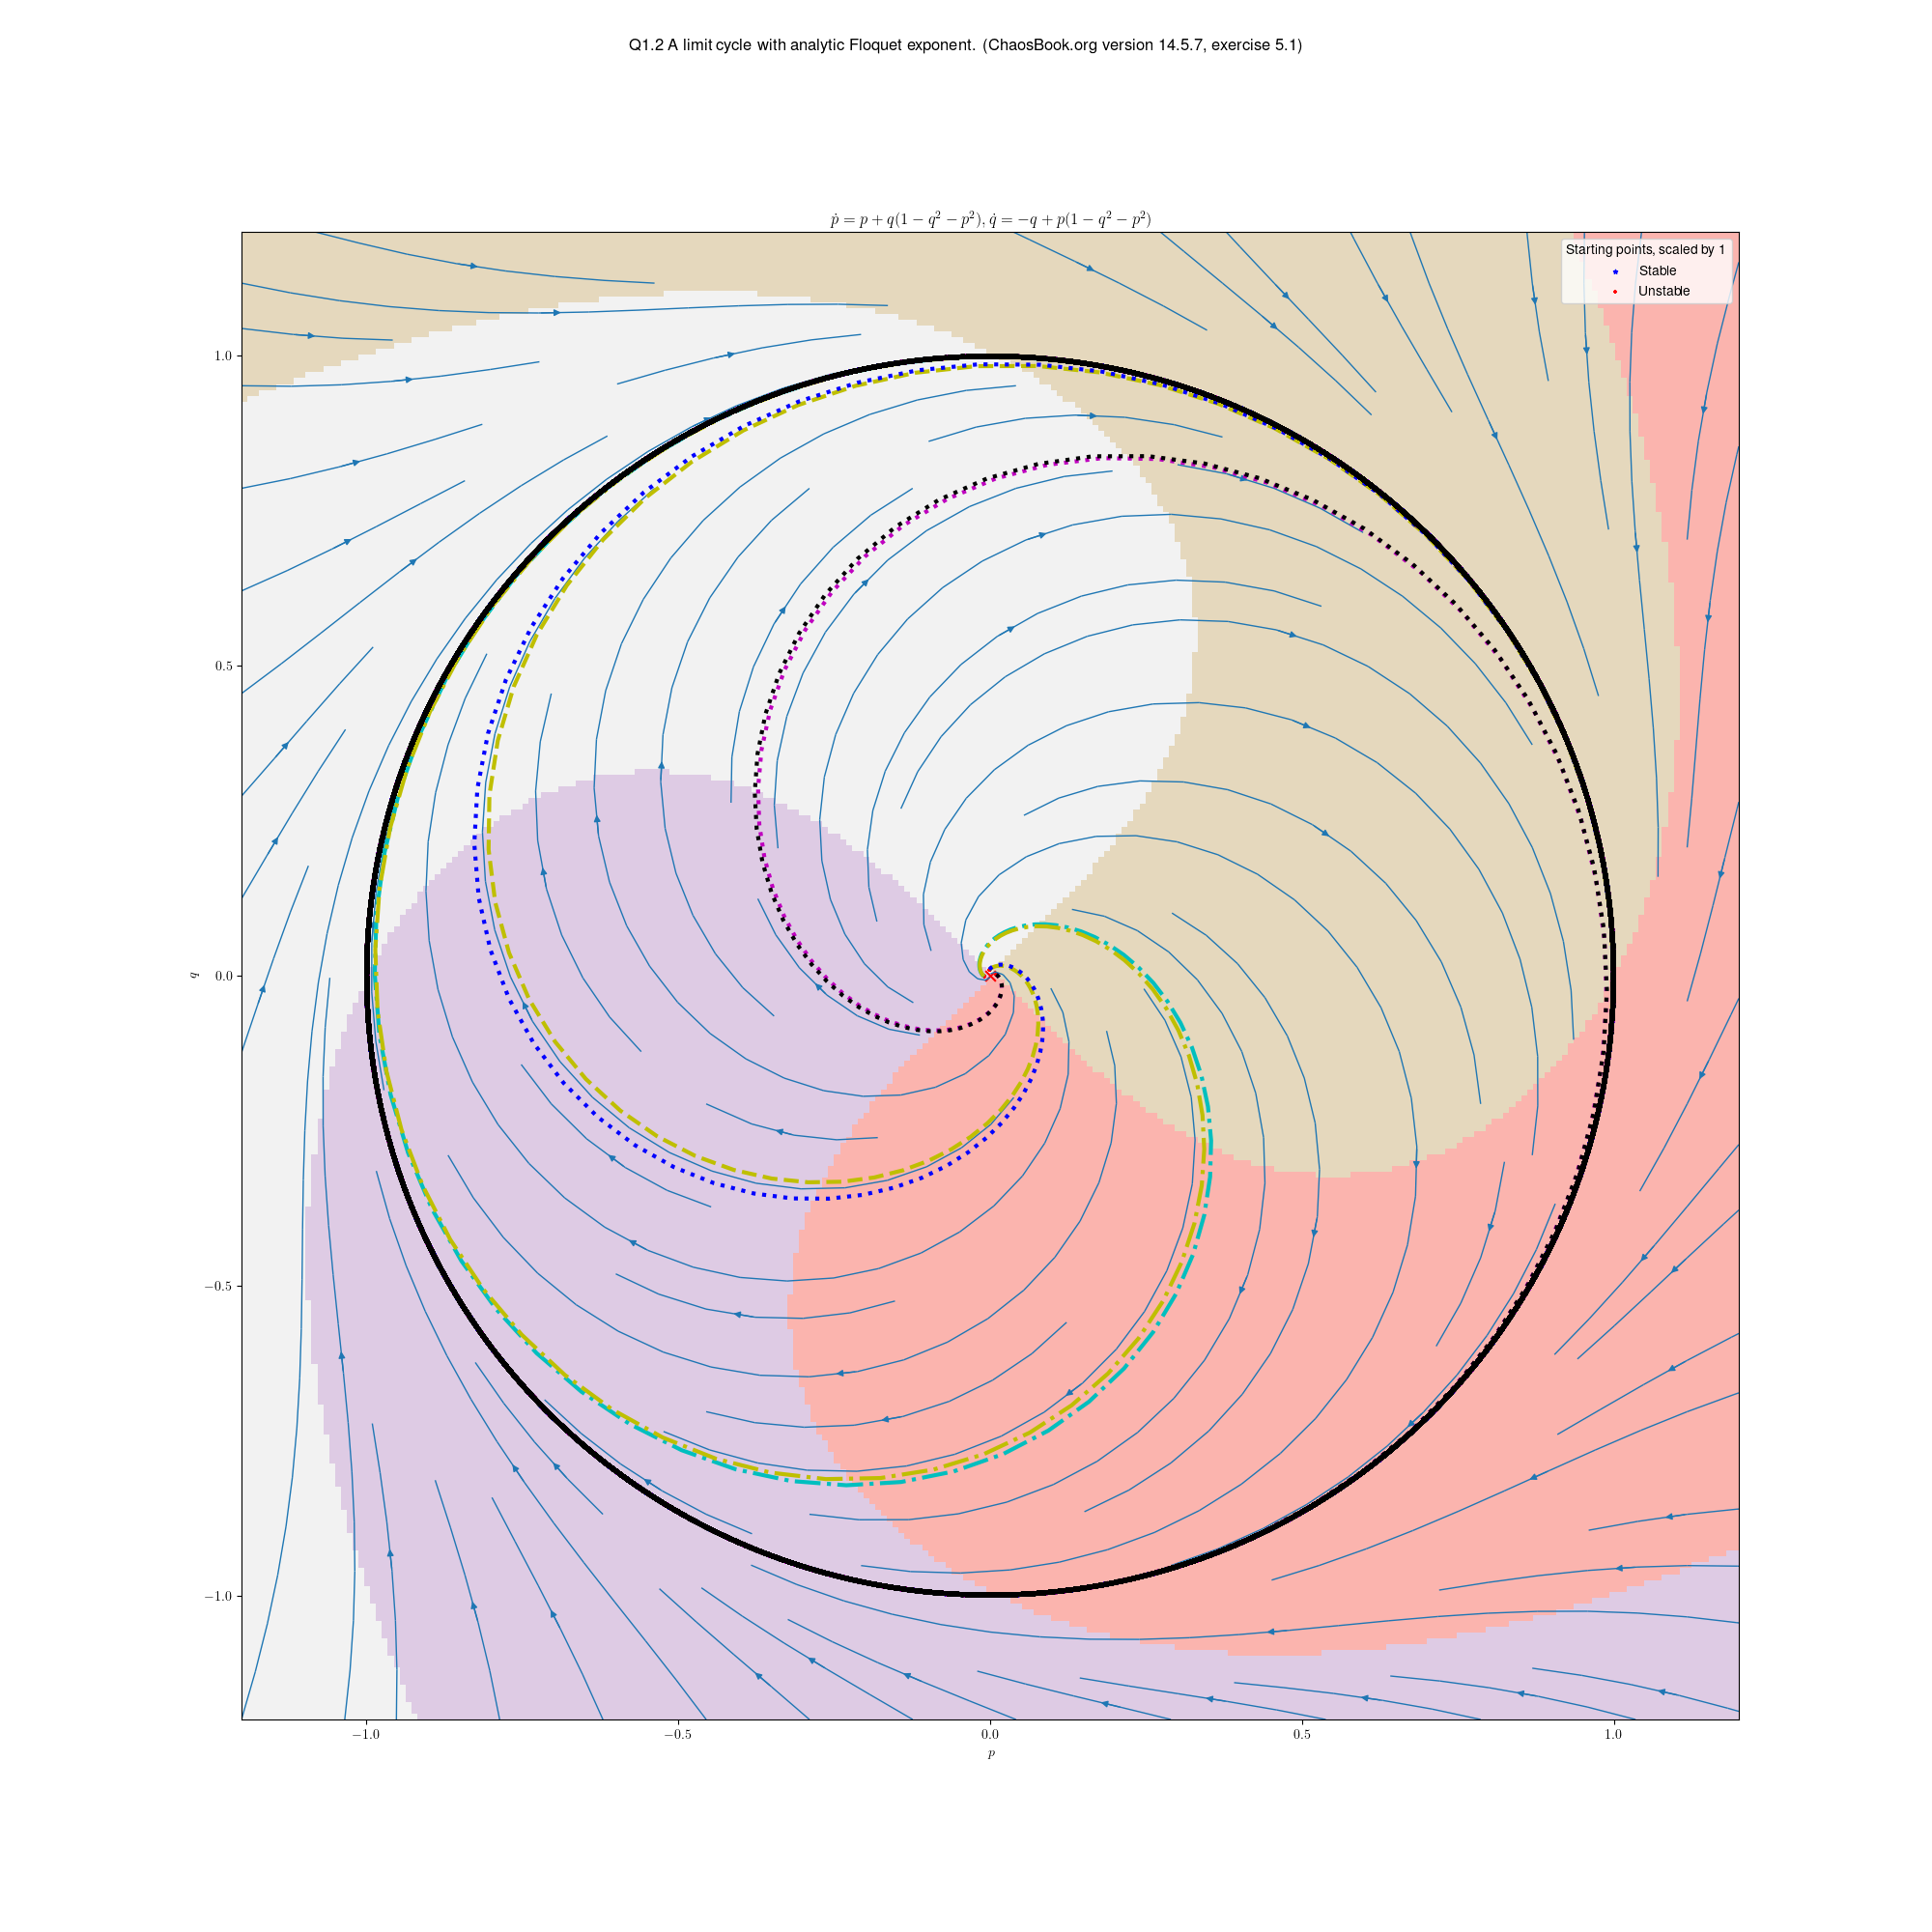
\includegraphics[width=\textwidth]{floquet.png}
\end{figure}
From \eqref{eq:dot_r0}
\begin{align*}
	\dot{r} =&	\cos{\theta} \dot{q} + \sin{\theta} \dot{p}\\
	=& 	\cos{\theta} \big[p + q\big(1-q^2-p^2\big)\big] + \sin{\theta} \big[-q + p\big(1-q^2-p^2\big)\big]\\
	=& 	\cos{\theta} \big[r \cancel{\sin{\theta}} + r \cos{\theta}\big(1-r^2\big)\big] + \sin{\theta} \big[\cancel{-r \cos{\theta}} + r \sin{\theta}\big(1-r^2\big)\big]\\
	=& r \big(1-r^2\big) \numberthis \label{eq:dot_r}
\end{align*}

Substitute $r=1+\delta r$ in \eqref{eq:dot_r}
\begin{align*}
	\dot{\delta} =& \big(1+\delta\big)\big(1 -1 -2 \delta - \delta^2\big)\\
	=& - \big(1+\delta\big) \delta (2 + \delta)\\
	\approxeq & - 2 \delta \text{, so}\\
	\delta(t) \propto & e^{-2 t}
\end{align*}
So the contracting Floquet exponent is $-2$.
\bibliographystyle{unsrt}
\addcontentsline{toc}{section}{Bibliography}
\bibliography{../../dynamics}
\end{document}
